\begin{name}
	{\tenchude}
	{Sở Phú Thọ - Lần 1}
	{LỚP TOÁN THẦY PHÁT}
	{{Cơ hội đến với tất cả mọi người nhưng để nắm bắt và đạt được thành công\\ thì phụ thuộc vào cách mà mỗi người trải nghiệm nó}}
\end{name}

\TN
\setcounter{ex}{0}
\Opensolutionfile{ans}[ans/ans-2-SoPhuTho-L1]
\begin{ex}%[12-EX-3-2026, Bùi Quang Phú]%[2D1N1-2]
\immini{Cho hàm số bậc ba $y=ax^3+bx^2+cx+d$ $(a\neq 0)$ có đồ thị như hình vẽ. Hàm số nghịch biến trên khoảng nào trong các khoảng sau đây?
	\choice
	{$(-\infty;-1)$}
	{\True $(-1;1)$}
	{$(1;+\infty)$}
	{$(-4;0)$}}{	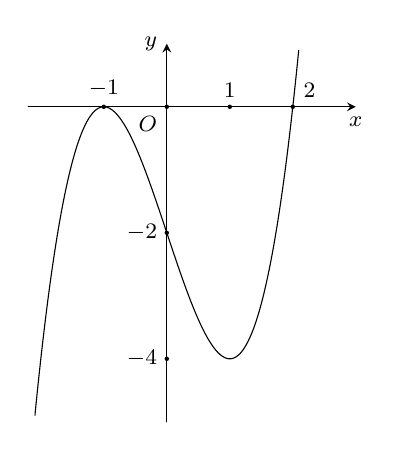
\begin{tikzpicture}[scale=0.8,font=\footnotesize,line join=round,line cap=round,>=stealth]
		\def\a{1} \def\b{0} \def\c{-3} \def\d{-2}% Hệ số
		\def\xmin{-2.2} \def\xmax{3}
		\def\ymin{-5} \def\ymax{1}
		%\draw[color=gray!50,dashed] (\xmin,\ymin) grid (\xmax,\ymax);
		\draw[->] (\xmin,0)--(\xmax,0) node [below]{$x$};
		\draw[->] (0,\ymin)--(0,\ymax) node [left]{$y$};
		\node at (0,0) [below left]{$O$};
		\node at (1,0) [above]{$1$};
		\node at (2,0) [shift=(45:0.3)]{$2$};
		\node at (0,-4) [left]{$-4$};
		\node at (0,-2) [left]{$-2$};
		\node at (-1,0) [above]{$-1$};
		\clip (\xmin+0.1,\ymin+0.1) rectangle (\xmax-0.5,\ymax-0.1);
		\draw[smooth,samples=300,domain=-2.1:2.15] plot(\x,{\a*(\x)^3+\b*(\x)^2+\c*(\x)+\d});
	\fill (-1,0) circle (1 pt);
		\fill (2,0) circle (1 pt);
			\fill (0,-2) circle (1 pt);
			\fill (0,-4) circle (1 pt);
		\fill (1,0) circle (1 pt);
	\fill (0,0) circle (1 pt);
		\end{tikzpicture}}
\loigiai{
Dựa vào đồ thị, ta thấy hàm số nghịch biến trên khoảng $(-1;1)$.
}
\end{ex}

\begin{ex}%[12-EX-3-2026, Bùi Quang Phú]%[1D1H5-3]
Nghiệm của phương trình $\sin x = \dfrac{\sqrt{3}}{2}$ là
	\choice
	{$x=\dfrac{\pi}{3}+k\pi; x=\dfrac{2\pi}{3}+k\pi, k \in \mathbb{Z}$}
	{$x=\pm\dfrac{\pi}{6}+k2\pi, k \in \mathbb{Z}$}
	{$x=-\dfrac{\pi}{6}+k2\pi; x=-\dfrac{5\pi}{6}+k2\pi, k \in \mathbb{Z}$}
	{\True $x=\dfrac{\pi}{3}+k2\pi; x=\dfrac{2\pi}{3}+k2\pi, k \in \mathbb{Z}$}
\loigiai{
Ta có $\sin x = \dfrac{\sqrt{3}}{2}\Leftrightarrow \sin x=\sin \dfrac{\pi}{3} \Leftrightarrow \hoac{& x=\dfrac{\pi}{3}+k2\pi \\& x=\dfrac{2\pi}{3}+k2\pi}~(k\in\mathbb{Z})$.
}
\end{ex}

\begin{ex}%[12-EX-3-2026, Bùi Quang Phú]%[1D2H3-3]
Cho cấp số nhân $(u_n)$ có số hạng đầu $u_1=3$, công bội $q=-2$. Số hạng thứ $5$ của cấp số nhân đó là
	\choice
	{$u_5=-96$}
	{$u_5=-5$}
	{\True $u_5=48$}
	{$u_5=23$}
\loigiai{Ta có $u_5=u_1\cdot q^4=3 \cdot (-2)^4=48$}
\end{ex}

\begin{ex}%[12-EX-3-2026, Bùi Quang Phú]%[0H9H4-1] 
Trong mặt phẳng $Oxy$, tâm của đường tròn $(C)\colon x^2+y^2+6x-4y-23=0$ có tọa độ là
	\choice
	{\True $(-3;2)$}
	{$(3;2)$}
	{$(3;-2)$}
	{$(-3;-2)$}
\loigiai{
Đường tròn $(C)\colon x^2+y^2+6x-4y-23=0$ có tâm $I$ với $x_I=\dfrac{6}{-2}=-3$ và $y_I=\dfrac{-4}{-2}=2$.\\
Vậy tâm của đường tròn $(C)$ là $I(-3;2)$.
}
\end{ex}

\begin{ex}%[12-EX-3-2026, Bùi Quang Phú]%[0D2H2-2]
\immini{Miền không bị gạch chéo trong hình vẽ (kể cả bờ) là miền nghiệm của hệ bất phương trình nào dưới đây?
	\choice
	{\True $\heva{& x\geq 0  \\& y\geq 0 \\& 2x+y\leq 4}$}
	{$\heva{& x\leq 0  \\& y\geq 0 \\& 2x+y\leq 4}$}
	{$\heva{& x\geq 0  \\& y\leq 0 \\& 2x-y\leq 4}$}
	{$\heva{& x\geq 0  \\& y\geq 0 \\& 2x-y\leq 4}$}}{\begin{tikzpicture}[scale=0.9, font=\footnotesize, line join=round, line cap=round,>=stealth]
		\def\xmin{-1.5}\def\xmax{4}
		\def\ymin{-1}\def\ymax{5}
		\draw[->] (\xmin,0)--(0,0)node[below left]{$O$}--(\xmax,0)node[below]{$x$};
		\draw[->] (0,\ymin)--(0,\ymax) node[left]{$y$};
		\clip (\xmin,\ymin) rectangle (\xmax,\ymax);
		\draw[smooth,samples=100]plot[domain=\xmin:\xmax](\x,{-2*(\x)+4});
		\fill[pattern=north east lines,opacity=.5] (-1/2,\ymax)--(\xmax,\ymax)--(\xmax,\ymin)--(5/2,\ymin);
		\fill[pattern=north east lines,opacity=.5] (-1/2,\ymax)--(\xmin,\ymax)--(\xmin,\ymin)--(0,\ymin)--(0,4)--cycle;
		\fill[pattern=north east lines,opacity=.5] (5/2,\ymin)--(2,0)--(0,0)--(0,\ymin)--cycle;
		\draw[fill=black]
		(2,0) circle(1pt) node[above right]{$2$} node[shift=(-135:0.3)]{$B$}
		(0,4) circle(1pt) node[left]{$4$} node[shift=(45:0.3)]{$A$};
		\fill (0,0) circle (1 pt);
		\end{tikzpicture}}
\loigiai{
Đường thẳng đi qua hai điểm $A(0;4)$ và $B(2;0)$ có phương trình $y=ax+b$.\\
Khi đó $\heva{& a\cdot 0+b=4  \\& 2a+b=0 \\}\Rightarrow \heva{&  a=-2 \\& b=4 \\}$. Suy ra $AB:y=-2x+4$ hay $2x+y-4=0$.\\
Ta nhận thấy điểm $(1;1)$ thuộc miền nghiệm.\\
Nên miền không bị gạch chéo trong hình vẽ (kể cả bờ) là miền nghiệm của hệ bất phương trình $\heva{& x\geq 0  \\& y\geq 0 \\& 2x+y\leq 4.}$
}
\end{ex}

\begin{ex}%[12-EX-3-2026, Bùi Quang Phú]%[2D1N2-1]
Điểm cực tiểu của hàm số $y=\dfrac{1}{3}x^3-2x^2+3x-1$ là
	\choice
	{$x=\dfrac{1}{3}$}
	{\True $x=3$}
	{$x=1$}
	{$x=-1$}
\loigiai{
Đạo hàm $y'=x^2-4x+3$. Ta có $y'=0 \Leftrightarrow \hoac{& x=1 \\& x=3.}$\\
Bảng biến thiên
\begin{center}
	
\begin{tikzpicture}
		\tkzTabInit[nocadre=false,lgt=1.2,espcl=2.5,deltacl=0.6]
		{$x$/0.6,$f'(x)$/0.6,$f(x)$/2}
		{$-\infty$,$1$,$3$,$+\infty$}
		\tkzTabLine{,+,$0$,-,$0$,+,}
		\tkzTabVar{-/$-\infty$,+/$f(1)$,-/$f(3)$,+/$+\infty$}
	\end{tikzpicture}
\end{center}
Vậy điểm cực tiểu của hàm số đã cho là $x=3$.
}
\end{ex}

\begin{ex}%[12-EX-3-2026, Bùi Quang Phú]%[2D1N4-1]
Đường thẳng nào dưới đây là đường tiệm cận xiên của đồ thị hàm số $y=2x-5+\dfrac{10}{x+3}$?
	\choice
	{\True $y=2x-5$}
	{$y=x+3$}
	{$y=2x$}
	{$y=2x+3$}
\loigiai{Đường tiệm cận xiên của đồ thị hàm số $y=2x-5+\dfrac{10}{x+3}$ là $y=2x-5$.}
\end{ex}

\begin{ex}%[12-EX-3-2026, Bùi Quang Phú]%[2D1H3-1]
Cho hàm số $y=\dfrac{3x+7}{x+1}$. Giá trị lớn nhất của hàm số đã cho trên đoạn $[0;3]$ bằng
	\choice
	{$3$}
	{\True $7$}
	{$4$}
	{$0$}
\loigiai{
Ta có $y'=\dfrac{-4}{(x+1)^2}>0$ với mọi $x\in[0;3]$.\\
Nên hàm số đã cho nghịch biến trên đoạn $[0;3]$.\\
Khi đó $\max\limits_{[0;3]} y=y(0)=7$.
}
\end{ex}

\begin{ex}%[12-EX-3-2026, Bùi Quang Phú]%[2H2N2-2]
Trong không gian $Oxyz$, điểm $A'$ đối xứng với điểm $A(2;-3;1)$ qua mặt phẳng $(Oxz)$ có tọa độ là
	\choice
	{$(-2;3;-1)$}
	{$(-2;-3;1)$}
	{$(2;-3;-1)$}
	{\True $(2;3;1)$}
\loigiai{
Điểm $A'$ đối xứng với điểm $A(2;-3;1)$ qua mặt phẳng $(Oxz)$ có tọa độ là $(2;3;1)$.
}
\end{ex}

\begin{ex}%[12-EX-3-2026, Bùi Quang Phú]%[2H2N2-3]
Trong không gian $Oxyz$, cho $\overrightarrow{a}=(1;2;3)$ và $\overrightarrow{b}=(0;-1;2)$. Vec-tơ $\overrightarrow{c}=\overrightarrow{a}-\overrightarrow{b}$ có tọa độ là
	\choice
	{$(-1;-3;-1)$}
	{\True $(1;3;1)$}
	{$(0;-2;6)$}
	{$(1;3;1)$}
\loigiai{Ta có $\overrightarrow{c}=\overrightarrow{a}-\overrightarrow{b}=(1;3;1)$.}
\end{ex}

\begin{ex}%[12-EX-3-2026, Bùi Quang Phú]%[2D3H1-3]
Thời gian truy cập Internet mỗi buổi tối của một nhóm học sinh được thống kê trong bảng sau
\begin{center}
\begin{tabular}{|c|c|c|c|c|c|}
\hline
Thời gian (phút) & $[10{,}5;12{,}5)$ & $[12{,}5;14{,}5)$ & $[14{,}5;16{,}5)$ & $[16{,}5;18{,}5)$ & $[18{,}5;20{,}5]$ \\
\hline
Số học sinh & $3$ & $12$ & $15$ & $24$ & $2$ \\
\hline
\end{tabular}
\end{center}
Khoảng tứ phân vị của mẫu số liệu đã cho bằng
	\choice
	{$\dfrac{83}{6}$}
	{$\dfrac{43}{3}$}
	{\True $\dfrac{19}{6}$}
	{$\dfrac{35}{2}$}
\loigiai{
Cỡ mẫu của mẫu số liệu ghép nhóm là $56$.\\
Sắp xếp mẫu số liệu ghép nhóm đã cho theo thứ tự không giảm là $x_1,x_2,\ldots,x_{56}$.\\
Ta có $\dfrac{56}{4} \cdot 1=14$. Ta thấy $x_{14} \in [12{,}5;14{,}5)$.\\
Tứ phân vị thứ nhất của mẫu số liệu ghép nhóm là
\[Q_1=12{,}5+\dfrac{14-3}{12} \cdot(14{,}5-12{,}5)=\dfrac{43}{3}.\]
Ta có $\dfrac{56}{4} \cdot 3=42$. Ta thấy $x_{42} \in [16{,}5;18{,}5)$.\\
Tứ phân vị thứ ba của mẫu số liệu ghép nhóm là
\[Q_1=16{,}5+\dfrac{42-(3+12+15)}{24} \cdot(18{,}5-16{,}5)=\dfrac{35}{2}.\]
Vậy khoảng tứ phân vị của mẫu liệu ghép nhóm là $\Delta Q=Q_3-Q_1=\dfrac{19}{6}$.
}
\end{ex}

\begin{ex}%[12-EX-3-2026, Bùi Quang Phú]%[2H2H1-3] 
Cho lăng trụ đều $ABC.A'B'C'$ có $AA'=3a$ và $AB=a$. Khi đó, cosin của góc giữa hai véc-tơ $\overrightarrow{AB'}$ và $\overrightarrow{A'C}$ bằng
	\choice
	{$\dfrac{7}{20}$}
	{$\dfrac{17}{20}$}
	{\True $-\dfrac{17}{20}$}
	{$-\dfrac{7}{20}$}
\loigiai{
\immini{Ta có $\overrightarrow{AB'}=\overrightarrow{AB}+\overrightarrow{AA'}$ và $\overrightarrow{A'C}=\overrightarrow{A'C'}+\overrightarrow{A'A}=\overrightarrow{AC}-\overrightarrow{AA'}$.\\
Khi đó 
\begin{eqnarray*}
	\overrightarrow{AB'}\cdot\overrightarrow{A'C}
	&=&\left(\overrightarrow{AB}+\overrightarrow{AA'}\right)
	\left(\overrightarrow{AC}-\overrightarrow{AA'}\right) \\
	&=&\overrightarrow{AB}\cdot\overrightarrow{AC}
	+\overrightarrow{AA'}\left(\overrightarrow{AC}-\overrightarrow{AB}\right)
	-\overrightarrow{AA'}^2 \\
	&=&\overrightarrow{AB}\cdot\overrightarrow{AC}
	+\overrightarrow{AA'}\cdot\overrightarrow{BC}
	-\left|\overrightarrow{AA'}\right|^2 \\
	&=&\left|\overrightarrow{AB}\right|\cdot\left|\overrightarrow{AC}\right|
	\cos\widehat{BAC}
	-\left|\overrightarrow{AA'}\right|^2 
	\quad (\text{vì } AA'\perp BC) \\
	&=&\dfrac{1}{2}a^2-(3a)^2 \\
	&=&\dfrac{-17a^2}{2}.
\end{eqnarray*}

Mặt khác $\left|\overrightarrow{AB'}\right|=\left|\overrightarrow{A'C}\right|=\sqrt{(3a)^2+a^2}=a\sqrt{10}$ (định lí Pythagore).\\
Do đó $\cos\left(\overrightarrow{AB'},\overrightarrow{A'C}\right)=\dfrac{\overrightarrow{AB'}\cdot\overrightarrow{A'C}}{\left|\overrightarrow{AB'}\right|\cdot\left|\overrightarrow{A'C}\right|}=-\dfrac{17}{20}$.

}{\begin{tikzpicture}[scale=1,font={\footnotesize}, >=stealth]	
	
	\path
	(0,0) coordinate (B)
	(1.3,-1.5) coordinate (A)
	(4,0) coordinate (C)
	($(A)+(0,3)$) coordinate (A')
	($(B)+(0,3)$) coordinate (B')
	($(C)+(0,3)$) coordinate (C')
	;
	\draw[dashed] (B)--(C) ;
	\draw (B)--(A)--(C) (A')--(B')--(C')--cycle (A)--(A') (B)--(B') (C)--(C')
	;
	% vẽ điểm
	\foreach \x/\g in {A/-90,B/180,C/0,B'/180,A'/90,C'/0}
	\draw[fill=black] (\x) circle (1pt)+(\g:.3)
	node{$\x$};	
		
\end{tikzpicture}}
	}
\end{ex}

\cauds
\begin{ex}%[Đào-V- Thuỷ]%[2D3H2-3]
	Một cơ sở sản xuất hàng thủ công thống kê về số lượng sản phẩm X bán được trong 30 ngày như sau
	\begin{center}
		\begin{tabular}{|c|c|c|c|c|c|}
			\hline
			Số lượng sản phẩm & $[100;140)$ & $[140;180)$ & $[180;220)$ & $[220;260)$ & $[260;300)$ \\
			\hline
			Số ngày & 3 & 6 & 12 & 6 & 3 \\
			\hline
		\end{tabular}
	\end{center}
	\choiceTF
	{\True Khoảng biến thiên của mẫu số liệu đã cho là $200$}
	{\True Khoảng tứ phân vị của mẫu số liệu đã cho là $60$}
	{Trung bình số sản phẩm bán được trong một ngày là $220$}
	{\True Phương sai của mẫu số liệu đã cho là $1\,920$}
	\loigiai
	{
		Bảng tần số tích luỹ
		\begin{center}
			\begin{tabular}{|c|c|c|c|c|c|}
				\hline
				Số lượng sản phẩm & $[100;140)$ & $[140;180)$ & $[180;220)$ & $[220;260)$ & $[260;300)$ \\
				\hline
				Số ngày & 3 & 6 & 12 & 6 & 3 \\
				\hline
				Tần số tích luỹ &3&9&21&27&30\\
				\hline
			\end{tabular}
		\end{center}
		\begin{itemchoice}
			\itemch Khoảng biến thiên của mẫu số liệu là $300-100=200$.
			\itemch Cỡ mẫu $n=30$.
			\begin{itemize}
				\item Ta có $\dfrac{n}{4}=7{,}5$ nên $Q_1$ thuộc nhóm $[140;180)$.
				\[
				Q_1= 140+ \dfrac{7{,}5-3}{6}\cdot 40= 170.
				\]
				\item Ta có $\dfrac{3n}{4}= 22{,}5$ nên $Q_3$ thuộc nhóm $[220;260)$.
				\[
				Q_3= 220+ \dfrac{22{,}5-21}{6}\cdot 40= 230.
				\] 
			\end{itemize}
			Khoảng tứ phân vị là $\Delta_Q= Q_3-Q_1= 230-170=60$.
			\itemch Trung bình số sản phẩm bán được trong một ngày là
			\[
			\overline{x}= \dfrac{120\cdot 3 + 160 \cdot 6 + 200 \cdot 12 + 240 \cdot 6 + 280 \cdot 3}{30}= 200.
			\]
			\itemch Phương sai của mẫu số liệu đã cho là
			\[
			s^2= \dfrac{(120-200)^2 \cdot 3 + (160-200)^2 \cdot 6 + (200-200)^2 \cdot 12+ (240-200)^2 \cdot 6 + (280-200)^2 \cdot 3}{30}= 1\,920.
			\]
		\end{itemchoice}
	}
\end{ex}

\begin{ex}%[Đào-V- Thuỷ]%[2D1H5-6]
	Cho hàm số $y=x^3-3x^2+5$ có đồ thị là $(C)$. Khi đó:
	\choiceTF
	{\True Hàm số đã cho nghịch biến trên khoảng $(0;2)$}
	{\True Hàm số đã cho có hai điểm cực trị}
	{Giá trị nhỏ nhất của hàm số đã cho trên khoảng $(0;+\infty)$ bằng $2$}
	{Tiếp tuyến của đồ thị $(C)$ tại điểm có hoành độ bằng $1$ là đường thẳng có phương trình $y=-3x+3$}
	\loigiai
	{
		Ta có $y'=3x^2-6x$, $y'=0 \Leftrightarrow \hoac{&x=0\\ &x=2.}$\\
		Bảng biến thiên
		\begin{center}
			
\begin{tikzpicture}
				\tkzTabInit[espcl=2.5,lgt=1.5,nocadre=false]
				{$x$/0.7,$y'$/0.7,$y$/2.5}
				{$-\infty$,$0$,$2$,$+\infty$}
				\tkzTabLine{,+,0,-,0,+,}
				\tkzTabVar{-/$-\infty$,+/$5$,-/$1$,+/$+\infty$}
			\end{tikzpicture}
		\end{center}
		Dựa vào bảng biến thiên ta được
		\begin{itemchoice}
			\itemch Hàm số đã cho nghịch biến trên khoảng $(0; 2)$.
			\itemch Hàm số đã cho có hai điểm cực trị tại $x=0$ và $x=2$.
			\itemch Giá trị nhỏ nhất của hàm số đã cho trên khoảng $(0; +\infty)$ bằng $1$ khi $x=2$.
			\itemch Với $x=1$ ta có $y(1)=3$ và $y'(1)=-3$.\\
			Phương trình tiếp tuyến của đồ thị $(C)$ tại điểm $(1;3)$ là
			\[
			y=-3(x-1)+3 \text{ hay } y=-3x+6.
			\]
		\end{itemchoice}
	}
\end{ex}

\begin{ex}%[Đào-V- Thuỷ]%[2H5V1-5]
	Cho hình chóp đều $S.ABCD$ có $SA=AB=4\sqrt{2}$. Gọi $M$ là trung điểm của $AB$, $G$ là trọng tâm tam giác $SAB$.
	\choiceTF
	{$\overrightarrow{SA}+\overrightarrow{SB}=\overrightarrow{SC}+\overrightarrow{SD}$}
	{\True $\overrightarrow{DS}=-2\overrightarrow{DM}+3\overrightarrow{DG}$}
	{\True Nếu chọn hệ tọa độ $Oxyz$ sao cho $O$ là tâm hình vuông $ABCD$, $B$ thuộc tia $Ox$, $C$ thuộc tia $Oy$, $S$ thuộc tia $Oz$. Điểm $E(a;b;c)$ thuộc mặt phẳng $(SBD)$ sao cho $C$, $E$, $G$ thẳng hàng thì $a+b+c=2$}
	{Nếu chọn hệ tọa độ $Oxyz$ sao cho $O$ là tâm hình vuông $ABCD$, $B$ thuộc tia $Ox$, $C$ thuộc tia $Oy$, $S$ thuộc tia $Oz$. Điểm $F(x;y;z)$ thuộc mặt phẳng $(SAC)$ sao cho $FG+FB$ nhỏ nhất thì $x+y+z=-1$}
	\loigiai
	{
		\begin{center}
			\begin{tikzpicture}[>=stealth,line join=round,line cap=round,font=\footnotesize,scale=0.8]
				\path 
				(0,0) coordinate (A)
				(-3,-2) coordinate (B)
				(5,0) coordinate (D)
				($(B)+(D)-(A)$) coordinate (C)
				($(A)!.5!(C)$) coordinate (O)
				($(O)+(90:5)$) coordinate (S)
				($(O)!1.2!(S)$) coordinate (z)
				($(O)!1.3!(B)$) coordinate (x)
				($(O)!1.7!(C)$) coordinate (y)
				($(A)!.5!(B)$) coordinate (M)
				($(S)!2/3!(M)$) coordinate (G)
				;
				\draw[] (S)--(B)--(C)--(D)--(S)--(C);
				\draw[dashed] (S)--(A)--(B)--(D)--(A)--(C) (G)--(D)--(M)--(S)--(O);
				\draw[->] (S)--(z) node[left] {$z$};
				\draw[->](B)--(x) node[below] {$x$};
				\draw[->](C)--(y) node[above right] {$y$}
				;
				\foreach \p/\g in {S/160, A/170, D/30, B/-90, C/-100, M/-60, O/-90, G/120}
				\draw[fill=black] (\p) circle (1pt) node[shift=(\g:2.5mm)] {$\p$};
			\end{tikzpicture}
		\end{center}
	\begin{itemchoice}
		\itemch Ta có $\overrightarrow{SA}+ \overrightarrow{SB} = \overrightarrow{SC} + \overrightarrow{SD} \Leftrightarrow \overrightarrow{SA}- \overrightarrow{SC}= \overrightarrow{SD}- \overrightarrow{SB} \Leftrightarrow \overrightarrow{CA}= \overrightarrow{BD}$ (vô lí).
		\itemch Vì $G$ là trọng tâm tam giác $SAB$ nên ta có
		\[
		\overrightarrow{SG}= 2\overrightarrow{GM} \Leftrightarrow \overrightarrow{DG}-\overrightarrow{DS} = 2 \left( \overrightarrow{DM}-\overrightarrow{DG}\right) \Leftrightarrow \overrightarrow{DS}= -2\overrightarrow{DM} + 3 \overrightarrow{DG}.
		\]
		\itemch Vì $ABCD$ là hình vuông có cạnh $AB=4\sqrt{2}$ nên $OA=OB=OC=OD=4$.\\
		Lại có $OS= \sqrt{SA^2-OA^2}= \sqrt{\left( 4\sqrt{2}\right)^2-4^2}=4$.\\
		Do đó ta được toạ độ các đỉnh $B(4;0;0)$, $C(0;4;0)$, $A(0;-4;0)$, $S(0;0;4)$.\\
		Vì $G$ là trọng tâm tam giác $SAB$ nên $G\left( \dfrac{4}{3}; -\dfrac{4}{3}; \dfrac{4}{3}\right)$.\\
		Ta có $S\in Oz$, $B \in Ox$, $D\in Ox$ nên $(SBD) \equiv (Ozx)$, suy ra $E(a;0;c)$.\\
		Mặt khác, vì $C$, $E$, $G$ thẳng hàng nên hai véc-tơ $\overrightarrow{CE}$, $\overrightarrow{CG}$ cùng phương.\\
		Ta có $\overrightarrow{CE}=(a;-4;c)$, $\overrightarrow{CG}= \left( \dfrac{4}{3}; -\dfrac{16}{3}; \dfrac{4}{3}\right)$. Do đó
		\[
		\dfrac{a}{\dfrac{4}{3}} = \dfrac{-4}{-\dfrac{16}{3}}=\dfrac{c}{\dfrac{4}{3}} \Rightarrow \heva{&a=1\\ &c=1} \Rightarrow a+b+c=2.
		\]
		\itemch 
		\begin{center}
			\begin{tikzpicture}[>=stealth,line join=round,line cap=round,font=\footnotesize,scale=.8]
				\path 
				(0,0) coordinate (a)
				(-2,-2) coordinate (b)
				(6,0) coordinate (d)
				($(b)+(d)-(a)$) coordinate (c)
				($(a)+(-60:1)$) coordinate (H)
				($(H)+(90:2.5)$) coordinate (B)
				($(H)!-1!(B)$) coordinate (B')
				($(a)+(-20:3)$) coordinate (F)
				($(B')!2!(F)$) coordinate (G)
				(intersection of a--d and B--H) coordinate (a1)
				(intersection of a--d and B--F) coordinate (a2)
				(intersection of a--d and G--F) coordinate (a3)
				(intersection of b--c and B--H) coordinate (b1)
				(intersection of b--c and G--F) coordinate (b2)
				;
				\draw[] (a)--(b)--(b1) (b2)--(c)--(d)--(a3) (a1)--(a)
				(H)--(B)--(F)--(G)--(B) (b1)--(B')--(b2)				
				;
				\draw[dashed] (a1)--(a3) (H)--(b1)--(b2)--(F);
				\foreach \p/\g in {B/90, H/180, B'/-90, F/-30, G/70}
				\draw[fill=black] (\p) circle (1pt) node[shift=(\g:3mm)] {$\p$};
				\begin{scope}
					\clip (a)--(b)--(c)--cycle;
					\draw (b) circle (1.2cm);
					\draw ($(b)+(15:22pt)$) node{$Oyz$};
				\end{scope}
			\end{tikzpicture}
		\end{center} 
		Ta thấy $S\in Oz$, $A, C \in Oy$ nên $(SAC) \equiv (Oyz)$ và hai điểm $B(4;0;0)$, $G\left( \dfrac{4}{3}; -\dfrac{4}{3}; \dfrac{4}{3}\right)$ nằm cùng phía so với mặt phẳng $(Oyz)$.\\
		Gọi $B'$ là điểm đối xứng của $B$ qua mặt phẳng $(Oyz)$, suy ra $B'(-4;0;0)$.\\
		Ta được $FG+FB= FG+FB' \ge GB'$. Dấu \lq\lq =\rq\rq\ xảy ra khi $F$ là giao điểm của $B'G$ và mặt phẳng $(Oyz)$.\\
		Do $F \in (Oyz)$ nên $F(0;x;y)$. Ta có $\overrightarrow{B'G}= \left( \dfrac{16}{3}; -\dfrac{4}{3}; \dfrac{4}{3}\right)$ và $\overrightarrow{B'F}= (4;y;z)$,\\
		Vì hai véc-tơ $\overrightarrow{B'G}$, $\overrightarrow{B'F}$ cùng phương nên ta được
		\[
		\dfrac{4}{\dfrac{16}{3}}= \dfrac{y}{-\dfrac{4}{3}} = \dfrac{z}{\dfrac{4}{3}} \Rightarrow \heva{&y=-1\\ &z=1} \Rightarrow x+y+z=0.
		\]
	\end{itemchoice}
	}
\end{ex}

\begin{ex}%[Đào-V- Thuỷ]%[2D1H5-8]
	Tại một khu bảo tồn thiên nhiên các nhà khoa học đã thả một số cá thể của một loài động vật quý hiếm trong một khu rừng rộng 10 hecta và theo dõi sự tăng trưởng số lượng của chúng. Họ thấy rằng số lượng cá thể của loài động vật đó sau $t$ năm kể từ khi nuôi tại khu bảo tồn được xấp xỉ bởi hàm số $h(t)=70\log_2\left(\dfrac{8t+1}{t+1}\right)+30$ (cá thể), $t$ là số thực dương và tốc độ tăng trưởng số lượng cá thể của loài động vật đó tại thời điểm sau đúng $t$ năm kể từ khi nuôi được xấp xỉ bởi hàm số $h'(t)$ (đơn vị: cá thể/năm).
	\choiceTF
	{\True Thời điểm ban đầu, người ta thả nuôi $30$ cá thể}
	{\True Sau 9 tháng kể từ khi bắt đầu nuôi, số lượng cá thể của loài động vật đó là $170$}
	{Tốc độ tăng trưởng số lượng cá thể của loài động vật đó tại thời điểm đúng $6$ năm kể từ khi nuôi là $\dfrac{10}{7}$ (cá thể/năm)}
	{\True Số lượng cá thể của loài động vật đó không vượt quá $240$}
	\loigiai
	{
		\begin{itemchoice}
			\itemch Số lượng cá thể thả nuôi tại thời điểm ban đầu là $h(0)=30$.
			\itemch Số lượng cá thể sau 9 tháng = $\dfrac{3}{4}$ năm là  $h\left( \dfrac{3}{4}\right)= 170$.
			\itemch Ta có $h'(t)= 70 \cdot \dfrac{\left( \dfrac{8t+1}{t+1}\right)'}{\dfrac{8t+1}{t+1} \cdot \ln 2}= \dfrac{490}{(t+1)(8t+1)\ln 2}$.\\
			Tốc độ tăng trưởng số lượng cá thể tại thời điểm $6$ năm kể từ khi nuôi là $h'(6)= \dfrac{10}{7 \ln 2}$.
			\itemch Ta có $h(t)=70 \log_2 \left( 8-\dfrac{7}{t+1}\right) + 30 < 70 \log_2 8 + 30 = 240$.\\
			Do đó số lượng cá thể không vượt quá $240$.
		\end{itemchoice}
	}
\end{ex}

\caukq
%\setcounter{ex}{0}
\begin{ex}%[12-EX-2-2026, Bùi Quang Phú]%[2H5V2-6]
Cho hình chóp $S.ABCD$ có đáy $ABCD$ là hình chữ nhật tâm $O$ với $AB=6$ và $AD=8$. Biết $SO$ vuông góc với mặt phẳng $(ABCD)$ và $SA$ tạo với mặt phẳng $(ABCD)$ một góc $45^\circ$. Gọi $M$ là trung điểm của $SA$. Biết khoảng cách giữa hai đường thẳng $SC$ và $DM$ bằng $\dfrac{120}{\sqrt{n}}$. Giá trị của $n$ bằng bao nhiêu?
\par\shortans[oly]{$1201$}
\loigiai{
\immini{Vì $ABCD$ là hình chữ nhật nên $AC=BD=\sqrt{6^2+8^2}=10$.\\
Vì $SA$ tạo với mặt phẳng $(ABCD)$ một góc $45^\circ$ nên $\widehat{SAO}=45^\circ$.\\
Khi đó $\triangle SAC$ vuông cân tại $S$. Suy ra $SO=\dfrac{AC}{2}=5$.\\
Đặt hệ trục tọa độ $Axyz$ như hình vẽ với
\[A(0;0;0),C(6;8;0),O(3;4;0),S(3;4;5),D(0;8;0),M\left(\dfrac{3}{2};2;\dfrac{5}{2}\right)\]
Ta có $\heva{& \overrightarrow{SC}=(3;4;-5) \\& \overrightarrow{DM}=\left(-\dfrac{3}{2};6;-\dfrac{5}{2}\right)  \\& \overrightarrow{CD}=(-6;0;0).}$\\
Suy ra khoảng cách giữa hai đường thẳng $SC$ và $DM$ là 
\[\mathrm{d}(SC,DM)=\dfrac{\left|\left[\overrightarrow{SC},\overrightarrow{DM}\right] \cdot \overrightarrow{CD}\right|}{\left|\left[\overrightarrow{SC},\overrightarrow{DM}\right]\right|}=\dfrac{\left|20\cdot(-6)\right|}{\sqrt{20^2+15^2+24^2}}=\dfrac{120}{\sqrt{1201}}.\]	
Vậy $n=1\,201$.
}{\begin{tikzpicture}[scale=0.9,font={\footnotesize}, >=stealth]	
		\path
		(0,0) coordinate (B)
		(4,0) coordinate (C)
		(2.2,1.35) coordinate (A)
		($(A)+(C)-(B)$) coordinate (D)
		(intersection of A--C and B--D) coordinate (O)
		($(O)+(0,3.2)$) coordinate (S)
		($(A)!1/2!(S)$) coordinate (M)
		;
		\draw[dashed] (B)--(A)--(D) (S)--(A) (A)--(C) (B)--(D)--(M) (S)--(O);
		\draw (B)--(C)--(D) (B)--(S)--(C)  (S)--(D) 
		;
		\draw[->] (A)--($(A)+(0,3.2)$)node[left]{$z$} ;
		\draw[->] (B)--($(A)!1.3!(B)$)node[left]{$x$} ;
		\draw[->] (D)--($(A)!1.2!(D)$)node[above]{$y$} ;
		% vẽ điểm
		\foreach \x/\g in {A/-90,B/180,C/-90,D/40,O/-90,S/90,M/160}
		\draw[fill=black] (\x) circle (1pt)+(\g:.3)
		node{$\x$};	
\end{tikzpicture}}
	}
\end{ex}

\begin{ex}%[Đào-V- Thuỷ]%[0D0V2-6]
	Cho đa giác đều 36 đỉnh $A_1$, $A_2$, $\ldots$, $A_{36}$ nội tiếp đường tròn tâm $O$. Chọn ngẫu nhiên 3 đỉnh trong số các đỉnh $A_1$, $A_2$, $\ldots$, $A_{36}$ của đa giác đã cho, biết xác suất để chọn được ba đỉnh tạo thành một tam giác có một góc bằng $120^\circ$ là $\mathrm{P}$. Giá trị biểu thức $595 \mathrm{P}$ bằng bao nhiêu?	
	\shortans[oly]{$33$}
	\loigiai
	{
		\immini
		{Số cách chọn tam giác có $3$ đỉnh trong $36$ đỉnh của đa giác đã cho là
		\[n(\Omega)= \mathrm{C}_{36}^3= 7140.\]
	Không mất tính tổng quát, đường tròn $(O)$ có góc ở tâm $\widehat{A_3OA_{15}}=120^\circ$.\\
	Nên số đo cung nhỏ $A_3A_{15}$ bằng $120^\circ$.\\
	Suy ra số đo cung lớn $A_3A_{15}$ bằng $360^\circ-120^\circ=240^\circ$.\\
	Do đó số đo của góc nội tiếp chắn cung lớn $A_3A_{15}$ bằng $120^\circ$ ($\widehat{A_3A_{11}A_{15}}=120^\circ$).\\
	Chọn bất kì các đỉnh $A_4,A_5,\ldots,A_{14}$ tạo với $A_3$ và $A_{15}$ một tam giác có góc $120^\circ$.\\
	Mặt khác, đa giác đều có $36$ đỉnh nên các góc $\widehat{A_iOA_{i+1}}=10^\circ$ với $i\in \left\{ 1; 2; \ldots; 35\right\}$.			
}{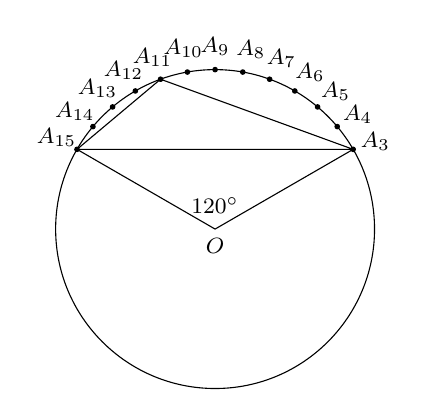
\begin{tikzpicture}[>=stealth,line join=round,line cap=round,font=\footnotesize,scale=.81]
			\def\r{2.5}
			\path (0,0) coordinate (O);
			\draw (O) circle (\r cm) node[below]{$O$};
			\foreach \x in {1,2,...,36}
			{\path (10*\x:\r) coordinate (A\x);
			}
			\foreach \x/\g in {3/20,4/30,5/40,6/50,7/60,8/70,9/90,10/100,11/110,12/120,13/130,14/140,15/150}
			\draw[fill=black] (A\x) circle (1pt) node[shift=(\g:3mm)] {$A_{\x}$};
			\draw (A3)--(O)--(A15)--cycle (A3)--(A11)--(A15);
			\draw (O) node[shift=(90:0.3)] {$120^\circ$};
			\end{tikzpicture}}
\noindent Gọi $A$ là biến cố: \lq\lq Chọn được ba đỉnh tạo thành tam giác có một góc bằng $120^\circ$\rq\rq. Ta có
\begin{itemize}
	\item Chọn góc tại tâm $O$ có số đo $120^\circ$, có $36$ cách (chẳng hạn góc $\widehat{A_3OA_{15}}=120^\circ$).
	\item Chọn đỉnh để tạo thành tam giác có một góc bằng $120^\circ$, có $11$ cách (gồm các đỉnh $A_4$, $A_5$, $\ldots$, $A_{14}$).
\end{itemize}
Do đó $n(A)= 36 \cdot 11= 396$. Suy ra $\mathrm{P}(A)= \dfrac{n(A)}{n(\Omega)}= \dfrac{396}{7140}= \dfrac{33}{595}$. Vậy $595 \mathrm{P}= 33$.
}
\end{ex}

\begin{ex}%[Khảo sát chất lượng toán 12 - Sở Phú Thọ (L1), Đình Nguyên]%[2H2V2-4]
	Cho hình chóp $S.ABC$, biết $SA$ vuông góc với mặt phẳng $(ABC)$ và $SA = 2\sqrt{3}$. Tam giác $ABC$ vuông tại $B$ với $AB = 6$, $BC = 8$. Gọi $M$ là trung điểm của $BC$. Giá trị của $\left|\overrightarrow{SA} + \overrightarrow{SB} + \overrightarrow{SC} + \overrightarrow{AM}\right| + \overrightarrow{SM} \cdot \overrightarrow{AB}$ bằng bao nhiêu?
\par\shortans[oly]{60} 
	\loigiai{
		\begin{center}
			\begin{tikzpicture}[scale=0.6, font=\footnotesize, line join=round, line cap=round, >=stealth]
				% Tọa độ các điểm dựa trên phép chiếu 
				\coordinate (B) at (0,0);
				\coordinate (C) at (5,0);
				\coordinate (A) at (-2,-1.5);
				\coordinate (S) at (-2,4);
				\coordinate (M) at ($(B)!0.5!(C)$);
				
				% Vẽ hệ trục tọa độ
				\draw[->] (C) -- (6.5,0) node[below] {$y$};
				\draw[->] (A) -- (-3,-2.25) node[right] {$x$};
				\draw[->] (0,20/7) -- (0,5) node[left] {$z$};
				\node[left] at (B) {$O$};
				\draw[dashed] (B)--(0,20/7);
				
				% Vẽ các cạnh hình chóp
				\draw[dashed] (S)--(B)--(C) (B)--(A) (A)--(M)--(S);
				\draw (S)--(A)--(C)--(S);
				
				% Đánh dấu điểm
				\foreach \p/\pos in {S/above, A/left, B/above right, C/below, M/above right}
				\draw[fill=black] (\p) circle (1pt) node[\pos]{$\p$};
			\end{tikzpicture}
		\end{center}
		Trong không gian $Oxyz$, chọn hệ trục tọa độ sao cho $B(0;0;0)$, $A(6;0;0)$, $C(0;8;0)$ như hình vẽ. \\
		Vì $SA \perp (ABC)$ và $SA = 2\sqrt{3}$ nên $S(6;0;2\sqrt{3})$.
		Vì $M$ là trung điểm của $BC$ nên $M(0;4;0)$.
		Ta có các véc-tơ sau
		\begin{itemize}
			\item $\overrightarrow{SA} = (0;0;-2\sqrt{3})$.
			\item $\overrightarrow{SB} = (-6;0;-2\sqrt{3})$.
			\item $\overrightarrow{SC} = (-6;8;-2\sqrt{3})$.
			\item $\overrightarrow{AM} = (-6;4;0)$.
		\end{itemize}
		Đặt $\overrightarrow{u} = \overrightarrow{SA} + \overrightarrow{SB} + \overrightarrow{SC} + \overrightarrow{AM} = (-18;12;-6\sqrt{3})$.\\
		Khi đó $\left|\overrightarrow{u}\right| = \sqrt{(-18)^2 + 12^2 + (-6\sqrt{3})^2} = \sqrt{324 + 144 + 108} = 24$.\\
		Mặt khác, $\overrightarrow{SM} = (-6;4;-2\sqrt{3})$ và $\overrightarrow{AB} = (-6;0;0)$.\\
		Suy ra $\overrightarrow{SM} \cdot \overrightarrow{AB} = (-6) \cdot (-6) + 4 \cdot 0 + (-2\sqrt{3}) \cdot 0 = 36$.\\
		Vậy giá trị biểu thức bằng $24 + 36 = 60$.
	}
\end{ex}

\begin{ex}%[Khảo sát chất lượng toán 12 - Sở Phú Thọ (L1), Đình Nguyên]%[2D1V3-6]
	Bác An có một cửa hàng chuyên bán buôn bưởi Đoan Hùng, bác nhận thấy rằng: Nếu bán mỗi kilogram bưởi với giá $30$ nghìn đồng thì mỗi tuần có $60$ đơn hàng và mỗi đơn hàng mua $100$ kilogram. Nếu cứ tăng giá mỗi kilogram bưởi thêm $2$ nghìn đồng thì hàng tuần số đơn hàng giảm $4$ đơn, đồng thời số lượng bưởi mà mỗi đơn hàng đặt mua cũng giảm đi $2$ kilogram. Hỏi bác cần bán mỗi kilogram bưởi với giá bao nhiêu nghìn đồng để lợi nhuận hàng tuần thu được là lớn nhất, biết giá nhập mỗi kilogram bưởi là $24$ nghìn đồng và giá bán không vượt quá $50$ nghìn đồng/$1$ kg. \textit{(Kết quả làm tròn đến hàng đơn vị).}
\par\shortans[oly]{40}
	\loigiai{
		Gọi $x$ là số lần tăng giá $2$ nghìn đồng ($x \ge 0$).\\
		Giá bán mỗi kilogram bưởi là $P = 30 + 2x$ (nghìn đồng).\\
		Theo giả thiết $P \le 50 \Rightarrow 30 + 2x \le 50 \Leftrightarrow x \le 10$.\\
		Số đơn hàng mỗi tuần là $60 - 4x$.\\
		Số kilogram bưởi mỗi đơn hàng là $100 - 2x$.\\
		Lợi nhuận hàng tuần là
		\begin{eqnarray*}
			f(x) &=& (P - 24) \cdot (60 - 4x) \cdot (100 - 2x) \\
			&=& (30 + 2x - 24)(60 - 4x)(100 - 2x) \\
			&=& 16(x + 3)(15 - x)(50 - x) \\
			&=& 16(x^3 - 62x^2 + 555x + 2\,250).
		\end{eqnarray*}
		Xét hàm số $f(x)$ trên đoạn $[0;10]$, ta có $f'(x) = 16(3x^2 - 124x + 555)$.\\
		Ta có $f'(x) = 0 \Leftrightarrow \hoac{&x_1 = \dfrac{62 - \sqrt{2179}}{3} \approx 5{,}11 \\ &x_2 = \dfrac{62 + \sqrt{2179}}{3} \approx 36{,}22 \text{ (loại).}}$\\
		Lập bảng biến thiên. 
		\begin{center}
			
\begin{tikzpicture}
				\tkzTabInit[nocadre=false,lgt=1.2,espcl=2.5,deltacl=0.6]
				{$x$ /0.6,$y’$ /0.6,$y$ /2}
				{ $0$, $x_1\approx 5{,}11$, $10$ } 
				\tkzTabLine{ , +, z, -, } 
				\tkzTabVar{ -/, + / , -/ } 
			\end{tikzpicture}
		\end{center}
		Ta thấy hàm số đạt cực đại tại $x \approx 5{,}11$.\\
		Giá bán tương ứng là $30 + 2 \cdot 5{,}11 = 40{,}22$ (nghìn đồng).
		Vậy bác An cần bán với giá khoảng $40$ nghìn đồng.
	}
\end{ex}

\begin{ex}%[Khảo sát chất lượng toán 12 - Sở Phú Thọ (L1), Đình Nguyên]%[1D1V5-6]
	Huyết áp là áp lực của máu tác động lên thành động mạch khi tim bơm máu vào động mạch. Giả sử trong một giai đoạn vận động thể thao, huyết áp của một người thay đổi theo thời gian được cho bởi hàm số $p(t) = 100 + 20 \cos(120\pi t)$, trong đó $p(t)$ là huyết áp tính theo đơn vị mmHg phụ thuộc vào thời gian $t$ tính theo phút. Trong $10$ phút tính từ thời điểm ban đầu khi $t = 0$, có bao nhiêu lần huyết áp của người này đạt mức $90$ mmHg?
\par\shortans[oly]{1200}
	\loigiai{
		Xét phương trình $p(t) = 90$ với $t \in [0;10]$. Ta có
		\begin{eqnarray*}
			100 + 20 \cos(120\pi t) = 90 &\Leftrightarrow& \cos(120\pi t) = -\dfrac{1}{2} \\
			&\Leftrightarrow& \hoac{&120\pi t = \dfrac{2\pi}{3} + k2\pi \\ &120\pi t = -\dfrac{2\pi}{3} + k2\pi} \Leftrightarrow \hoac{&t = \dfrac{1}{180} + \dfrac{k}{60} \\ &t = -\dfrac{1}{180} + \dfrac{k}{60}} (k \in \mathbb{Z}) \text{.}
		\end{eqnarray*}
		\begin{itemize}
			\item Với $t = \dfrac{1}{180} + \dfrac{k}{60} \in [0;10] \Rightarrow -\dfrac{1}{3} \le k \le \dfrac{1799}{3} \Rightarrow k \in \{0; \dots; 599\}$ (600 giá trị).
			\item Với $t = -\dfrac{1}{180} + \dfrac{k}{60} \in [0;10] \Rightarrow \dfrac{1}{3} \le k \le \dfrac{1801}{3} \Rightarrow k \in \{1; \dots; 600\}$ (600 giá trị).
		\end{itemize}
		Vậy có tổng cộng $1200$ lần huyết áp đạt mức $90$ mmHg.
	}
\end{ex}

\begin{ex}%[Khảo sát chất lượng toán 12 - Sở Phú Thọ (L1), Đình Nguyên]%[1H8V7-4]
	Cho hình lăng trụ $ABC.A'B'C'$ có $A'A = A'B = A'C$, cạnh bên $AA' = 4$, đáy $ABC$ là tam giác đều. Biết mặt phẳng $(BCC'B')$ tạo với mặt phẳng $(ABC)$ một góc $60^{\circ}$. Thể tích của khối lăng trụ đã cho bằng bao nhiêu?
\par\shortans[oly]{18}
	\loigiai{
		\begin{center}
			\begin{tikzpicture}[scale=0.7, font=\footnotesize, line join=round, line cap=round, >=stealth]
				\coordinate (A) at (0,0);
				\coordinate (B) at (1.6,-2.1);
				\coordinate (C) at (4,0);
				\coordinate (M) at ($(B)!0.5!(C)$);
				\coordinate (G) at ($(A)!2/3!(M)$); 
				\coordinate (A') at ($(G)+(0,4)-(A)$);
				\coordinate (B') at ($(A')+(B)-(A)$);
				\coordinate (C') at ($(A')+(C)-(A)$);
				\coordinate (M') at ($(B')!0.5!(C')$);
				\draw[dashed] (A')--(G) (G)--(A) (G)--(B) (G)--(C) (A)--(C) (G)--(M)--(A');
				\draw (A)--(B)--(C) (A')--(B')--(C')--cycle (A')--(A) (B')--(B) (C')--(C) (A')--(M')--(M);
				\foreach \p/\pos in {A/left, B/below, C/right, A'/above, B'/left, C'/right, G/below left, M/right, M'/above}
				\draw[fill=black] (\p) circle (1pt) node[\pos]{$\p$};
			\end{tikzpicture}
		\end{center}
		Gọi $G$ là tâm đường tròn ngoại tiếp tam giác đều $ABC$. Vì $A'A=A'B=A'C$ nên $A'G \perp (ABC)$.\\
		Gọi $M$, $M'$ lần lượt là trung điểm của $BC$, $B'C'$.\\
		Ta có $\heva{&BC\perp AM\\&BC\perp AG}\Rightarrow BC\perp (AMM'A')\Rightarrow BC\perp MM'$.\\
		Khi đó góc giữa $(BCC'B')$ và $(ABC)$ bằng góc giữa $AM$ và $MM'$.\\
		Mà $MM'\parallel AA'$ nên suy ra $(AM,MM')=(AM,AA')=\widehat{A'AG} = 60^{\circ}$.\\
		Trong $\triangle A'GA$ vuông tại $G$, ta có
		\begin{itemize}
			\item $AG = AA' \cdot \cos 60^{\circ} = 4 \cdot \dfrac{1}{2} = 2$.
			\item $h = A'G = AA' \cdot \sin 60^{\circ} = 4 \cdot \dfrac{\sqrt{3}}{2} = 2\sqrt{3}$.
		\end{itemize}
		Đặt cạnh đáy là $a$. Vì $G$ là tâm tam giác đều $ABC$ nên $AG = \dfrac{a\sqrt{3}}{3} \Rightarrow 2 = \dfrac{a\sqrt{3}}{3} \Rightarrow a = 2\sqrt{3}$.\\
		Diện tích đáy $S_{ABC} = \dfrac{a^2\sqrt{3}}{4} = \dfrac{(2\sqrt{3})^2\cdot \sqrt{3}}{4} = 3\sqrt{3}$.\\
		Thể tích khối lăng trụ $V = S_{ABC} \cdot A'G = 3\sqrt{3} \cdot 2\sqrt{3} = 18$.
	}
\end{ex}  
\Closesolutionfile{ans}
% \indapan{4}{ans/ans-2-SoPhuTho-L1}


